% \appendix
% Technical appendices with additional results, figures, graphs, and proofs may be submitted with the paper submission before the full submission deadline (see above). You can upload a ZIP file for videos or code, but do not upload a separate PDF file for the appendix. There is no page limit for the technical appendices. 

% Note: Think of the appendix as ``optional reading'' for reviewers. The paper must be able to stand alone without the appendix; for example, adding critical experiments that support the main claims to an appendix is inappropriate.
\newpage
\section{Counterexample for initial-visit MCES with non-greedy bias}
\label{app: non greedy}

Bertsekas and Tsitsiklis show in \cite[Example~5.12]{Bertsekas1996Neuro-DynamicProgramming} that IV MCES can converge to suboptimal solutions when greedy actions are updated less frequently than non-greedy actions.
The single-state MDP in \autoref{fig: experiment off-policy bias MDP} is the simplest such example.

Episodes are initialised to favour the non-greedy action,
meaning
when $q_k(s,\pi_*(s)) \ge q_k(s,\bar\pi(s))$
the initial state-action pair is $(s,\pi_*(s))$ with a small probability $\epsilon$ and $(s,\bar\pi(s))$ with probability $1-\epsilon$,
with the probabilities reversed otherwise.
% Alternatively, when
% $q_k(s,\pi_*(s)) < q_k(s,\bar\pi(s))$
% we initialise each episode in $(s,\pi_*(s))$ with probability $\epsilon$, or in $(s,\bar\pi(s))$ with probability $1-\epsilon$

\autoref{fig: experiment for off-policy bias} shows simulations with $\epsilon = 0.1$. The streamlines indicate the mean-field flow.
Solutions starting to the right of the separatrix typically converge to $q_{\pi_*}$, whereas those starting to the left leave the optimal region $Q(\pi_*)$ and converge to a boundary point.

% solutions which start in the region of the optimal policy, below the boundary, can leave it when to the left of the indicated separatrix, and converge to a point on the boundary which has the property that outflow and inflow are in opposite directions.   

\begin{figure}[htbp]
    \centering
    % \hrule
    % \vspace{0.4cm}

    \begin{subfigure}[b]{0.3\textwidth}
        \centering
        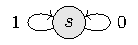
\includegraphics{figures/counter-mdp.pdf}
        % \begin{tikzpicture}[
        %     scale=1, auto, node distance=2cm, 
        %     every edge/.style={draw, <-, font=\small},
        %     state/.style={circle, fill=mylightgrey, draw=black, text=black}
        % ]
        %     % Nodes
        %     \node[state] (s1) at (0,0) {$s$};
        %     % Edges
        %     \path[->]
        %         (s1) edge[out=160, in=200, loop, looseness=8, draw=black] node[pos=0.5, left, text=black] {1} (s1)
        %         (s1) edge[out=20, in=340, loop, looseness=8, draw=black] node[pos=0.5, right, text=black] {0} (s1) ;
        %         % (s1) edge[out=145, in=215, loop, looseness=7] 
        %         %     node[pos=0.5, right] {$\best{a}$} 
        %         %     node[pos=0.5, left] {1} 
        %         % (s1)
        %         % (s1) edge[out=35, in=325, loop, looseness=7] 
        %         %     node[pos=0.5, left] {$\worst{a}$} 
        %         %     node[pos=0.5, right] {0} 
        %         % (s1);
        % \end{tikzpicture}
        \caption{MDP}
        \label{fig: mdp for unconditional experiment}
    \end{subfigure}%
    \hfill
    \begin{subfigure}[b]{0.3\textwidth}
        \centering
        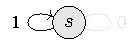
\includegraphics{figures/counter-mdp-opt.pdf}
        % \begin{tikzpicture}[
        %     scale=1, auto, node distance=2cm, 
        %     every edge/.style={draw, <-, font=\small},
        %     state/.style={circle, fill=mylightgrey, draw=black, text=black}
        % ]
        %     % Nodes
        %     \node[state] (s1) at (0,0) {$s$};
        %     % Edges
        %     \path[->]
        %         (s1) edge[out=160, in=200, loop, looseness=8, draw=black] node[pos=0.5, left, text=black] {1} (s1)
        %         (s1) edge[out=20, in=340, loop, looseness=8, draw=mylightgrey] node[pos=0.5, right, text=mylightgrey] {0} (s1) ;
        %         % (s1) edge[out=160, in=200, loop, looseness=8] node[pos=0.5, left] {$\begin{aligned}
        %         %     & \best{a} \\
        %         %     & 1
        %         % \end{aligned}$} (s1)
        %         % (s1) edge[out=20, in=340, loop, looseness=8, draw=mylightgrey] node[pos=0.5, right, text=mylightgrey] {$\begin{aligned}
        %         %     & \worst{a} \\
        %         %     & 0
        %         % \end{aligned}$} (s1);
        % \end{tikzpicture}
        \caption{Policy $\best{\pol}$}
    \end{subfigure}%
    \hfill
    \begin{subfigure}[b]{0.3\textwidth}
        \centering
        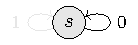
\includegraphics{figures/counter-mdp-worst.pdf}
        % \begin{tikzpicture}[
        %     scale=1, auto, node distance=2cm, 
        %     every edge/.style={draw, <-, font=\small},
        %     state/.style={circle, fill=mylightgrey, draw=black, text=black}
        % ]
        %     % Nodes
        %     \node[state] (s1) at (0,0) {$s$};
        %     % Edges
        %     \path[->]
        %         (s1) edge[out=160, in=200, loop, looseness=8, draw=mylightgrey] node[pos=0.5, left, text=mylightgrey] {1} (s1)
        %         (s1) edge[out=20, in=340, loop, looseness=8, draw=black] node[pos=0.5, right, text=black] {0} (s1) ;
        %         % (s1) edge[out=160, in=200, loop, looseness=8, draw=mylightgrey] node[pos=0.5, left, text=mylightgrey] {$\begin{aligned}
        %         %     & \best{a} \\
        %         %     & 1
        %         % \end{aligned}$} (s1)
        %         % (s1) edge[out=20, in=340, loop, looseness=8] node[pos=0.5, right] {$\begin{aligned}
        %         %     & \worst{a} \\
        %         %     & 0
        %         % \end{aligned}$} (s1);
        % \end{tikzpicture}
        \caption{Policy $\worst{\pol}$}
    \end{subfigure}%
    
    \caption{MDP that exhibits a stable suboptimal solution for IV MCES when updates are biased towards non-greedy actions.}
    \label{fig: experiment off-policy bias MDP}
\end{figure}

\begin{figure}[htbp]
    \centering
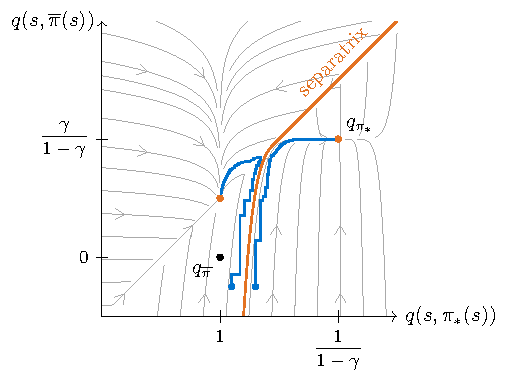
\includegraphics{figures/simple-counter.pdf}
   %  \pgfmathsetmacro{\ticklen}{0.1}
   %  \pgfmathsetmacro{\xmin}{-1}
   %  \pgfmathsetmacro{\xmax}{4}
   %  \pgfmathsetmacro{\ymin}{-1}
   %  \pgfmathsetmacro{\ymax}{4}
    
   %  \pgfmathsetmacro{\qbpolx}{3}
   %  \pgfmathsetmacro{\qbpoly}{2}
   %  \pgfmathsetmacro{\qwpolx}{1}
   %  \pgfmathsetmacro{\qwpoly}{0}

    
   % %\begin{subfigure}[b]{0.9\textwidth}
   % %    \centering

   %      \begin{tikzpicture}[scale=1]

   %          \pgfmathsetmacro{\eps}{0.9}
   %          \pgfmathsetmacro{\mbpolx}{1-\eps}
   %          \pgfmathsetmacro{\mbpoly}{\eps}
   %          \pgfmathsetmacro{\mwpolx}{\eps}
   %          \pgfmathsetmacro{\mwpoly}{1-\eps}
        
   %          \pgfmathsetmacro{\qc}{(\mbpolx*\qbpolx - \mbpoly*\qbpoly)/(\mbpolx - \mbpoly)}
        
   %          % Add the streamline plot using pgfplots
   %          \begin{axis}[
   %              hide axis,
   %              xmin=\xmin, xmax=\xmax,
   %              ymin=\ymin, ymax=\ymax,
   %              width=5cm, % Scale the width to match your scaling
   %              height=5cm, % Adjust for aspect ratio
   %              clip=true, % Hide parts of streamlines outside the axes
   %              scale only axis,
   %              xshift=-1cm, % Custom shift in x-direction
   %              yshift=-1cm % Custom shift in y-direction
   %          ] 
   %              \addplot[mygrey, no marks] 
   %              table [ x expr=\thisrowno{0}, 
   %                      y expr=\thisrowno{1}, 
   %                      col sep=comma, 
   %                      unbounded coords=jump] 
   %              {figures/32/streamlines-strong-off-policy.csv};

   %              \addplot[CambridgeCoreBlue, no marks, line width=0.3mm] 
   %              table [ x expr=\thisrowno{0}, 
   %                      y expr=\thisrowno{1}, 
   %                      col sep=comma, 
   %                      unbounded coords=jump] 
   %              {figures/32/simulations-strong-off-policy.csv};
    
   %              \addplot[
   %                  smooth,
   %                  line width=0.3mm,
   %                  CambridgeCoreOrange,
   %                  domain=-4:0,
   %                  samples=10
   %              ] plot ( 
   %                  {\qc + (1 - exp(-\mbpolx*x)) * (\qbpolx - \qc)}, 
   %                  {\qc + (1 - exp(-\mbpoly*x)) * (\qbpoly - \qc)}
   %              );
   %              \addplot[
   %                  smooth,
   %                  line width=0.3mm,
   %                  CambridgeCoreOrange,
   %                  domain=0:1,
   %                  samples=2
   %              ] plot ( 
   %                  {x*\qc + (1 - x) * \xmax}, 
   %                  {x*\qc + (1 - x) * \ymax}
   %              );
   %          \end{axis}
    
   %          % Draw the grid and axes
   %          \draw[->] (\xmin,\ymin) -- (\xmax,\ymin) node[right] {$q(s,\best{\pol}(s))$};
   %          \draw[->] (\xmin,\ymin) -- (\xmin,\ymax) node[left] {$q(s,\worst{\pol}(s))$};
   %          % \draw (\xmin,\ymax) -- (\xmax,\ymax) ;
   %          % \draw (\xmax,\ymin) -- (\xmax,\ymax) ;
    
   %          % Draw the line y = x
   %          % \draw[black, dotted] (\xmin,\ymin) -- (\xmax,\ymax);
    
   %          % Add labels to the axes
   %          \draw (\qbpolx,\ymin+\ticklen) -- (\qbpolx,\ymin-\ticklen) node[below, font=\small] {$\dfrac{1}{1-\discount}$};
   %          \draw (\xmin+\ticklen,\qbpoly) -- (\xmin-\ticklen,\qbpoly) node[left, font=\small] {$\dfrac{\discount}{1-\discount}$};
   %          \draw (\qwpolx,\ymin+\ticklen) -- (\qwpolx,\ymin-\ticklen) node[below, font=\small] {$1$};
   %          \draw (\xmin+\ticklen,\qwpoly) -- (\xmin-\ticklen,\qwpoly) node[left, font=\small] {0};
    
   %          % Add the points with associated text
   %          \filldraw[fill=CambridgeCoreOrange, draw=CambridgeCoreOrange] (\qbpolx,\qbpoly) circle (1.5pt) node[above right, text=black] {$q_{\best{\pol}}$};
   %          \filldraw[fill=black, draw=black] (\qwpolx,\qwpoly) circle (1.5pt) node[below left, text=black] {$q_{\worst{\pol}}$};
   %          \filldraw[fill=CambridgeCoreOrange, draw=CambridgeCoreOrange] (\qwpolx,\qwpolx) circle (1.5pt) ;
   %          \filldraw[fill=CambridgeCoreBlue, draw=CambridgeCoreBlue] (1.2, -0.5) circle (1.5pt) ;
   %          \filldraw[fill=CambridgeCoreBlue, draw=CambridgeCoreBlue] (1.6, -0.5) circle (1.5pt) ;
   %          \node at (\xmax-0.25,\ymax-0.25) [anchor=south east, rotate=45, text=CambridgeCoreOrange] {separatrix};
    
   %      \end{tikzpicture}
    %\end{subfigure}%
    % \vspace{0.3cm}
    \caption{The streamlines of the mean-field flow indicate that there are two basins of attraction when the non-greedy bias is large ($\epsilon = 0.1$).
    Solutions starting to the left of the separatrix tend to converge to a suboptimal fixed point on the boundary when the learning rates are sufficiently small.
    Those starting to the right converge to $\qopt$. The two simulations of MCES in blue confirm this conclusion.}
    \label{fig: experiment for off-policy bias}
        \label{fig: experiment for off-policy bias large}
\end{figure}
